\chapter{神经网络处理器编译器验证思路}

在阐明验证思路之前,我们应首先来熟悉一下神经网络处理器的软件构架, 如\autoref{fig:Software stock}所示,神经网络处理器的软件部分自上而下主要分成如下几个层次:

1.User Program:上层应用,即程序员基于编程框架。定义特定的神经网络结构来实现特定的神经网络功能。

2.Framework:编程框架,相当于连接的桥梁。例如(Caffe、TensorFlow),为用户提供神经网络基本操作,减轻程序员的编程负担,是一种编程工具。

3.runtime library:库是一个屏蔽掉底层硬件,编译器、启动程序的具体信息,对上层编程框架提供神经网络原子(即神经网络的某一层,这是神经网络最基本的组成单元)操作的编程接口的系统软件。

4.driver、compile:编译器,将上层的库传来的指令描述符按照神经网络处理器的指令集翻译成能接受的机器指令。驱动:对上层库提供调用底层硬件最基本的操作支持,例如读取数据、启动关闭、读取寄存器等。

5.hardware 硬件:即神经网络处理器(DaDianNao)

\begin{figure}[!htbp]
\centering
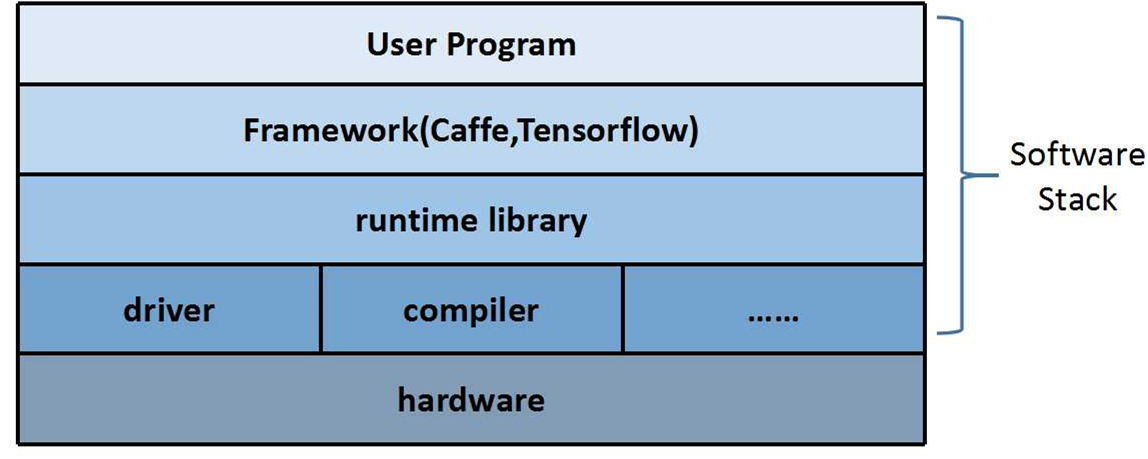
\includegraphics[width=12cm]{Software_stock.jpg}
\caption{神经网络处理器的软件架构}
\label{fig:Software stock}
\end{figure}

验证需要对变量进行控制,由于我们需要验证的是神经网络处理器的编译器,因此主要关注的是库(runtime library)以及编译器(compiler)的正确性。

对于神经网络处理器编译器的验证流程,可以概括为如下几个步骤,首先,生成包含有网络参数与结构信息的配置文件prototxt 。接着,根据prototxt调用caffe提供的接口生成具有训练参数的神经网络模型caffemodrel,然后调用caffe框架,经过一系列的内存分配,指令生成的操作后,调用库的接口,获得神经网络处理器结果,将这个结果caffe中生成的cpu结果进行比对,以达到验证目的。

\section{protext的生成}
要运行caffe,首先需要先创建一个模型(model),caffe里自带了不少常用的神经网络模型,而一个模型由多个层(layer)构成,每一个层又包含多个参数,每一个层的参数都定义在caffe.proto这个文件内。因此,想要生成一个可以用于验证的模型,我们必须首先生成一个符合结构要求并含有参数定义的prototxt。

我们自己编写了一套随机网络生成器,通过这个随机网络生成器,我们可以根据用户的需求,生成结构随机,参数随机且具有正确合理的连接方式的神经网络。同时,这个生成器也可以根据用户需求,生成包含有指定层序列、甚至是结构固定的网络,同时,我们也搭建了一个数据库,分三个层次将一些网络的样例加入数据库中。关于随机网络生成器的细节将在第三章详细概述。
\section{caffe\underline{ }model的创建}
调用caffe提供的caffe\underline{ }param接口(caffe\underline{ }param是caffe提供的一个记录网络结构与权值并能直接生成caffe\underline{ }model的类),初始化一个Net类,在Net中我们将权值初始化,再赋值传回param类中,而后net\underline{ }param可以直接将网络结构以及权值写入caffe\underline{ }model中,我们便生成一个具有随机权值的真实网络。

\section{caffe重载}
caffe是一个快速的深度学习框架,现在只能调用cpu与gpu进行计算。因此,为了让caffe能够调用神经网络处理器进行运算,我们对caffe进行了移植,在框架下加入对神经网络处理器硬件的支持。把原来的cpu操作,重载成为神经网络处理器的指令,成为库能接受的操作和运算。

从实现上来看,即将操作的xxx\underline{ }Forward\underline{ }cpu改写为支持神经网络处理器运算的xxx\underline{ }Forward\underline{ }ipu。同时,我们也在内存调度与空间管理等细节上进行了完善,使得caffe可以支持神经网络处理器的运算。

\section{caffe运行ipu的过程}
\begin{figure}[!htbp]
\centering
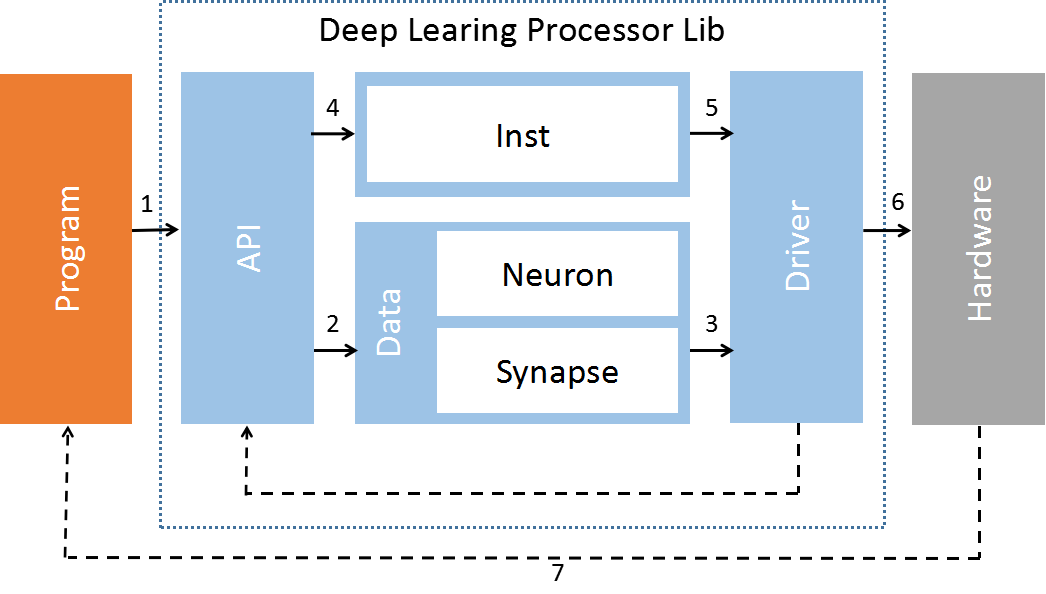
\includegraphics[width=12cm]{DLP1.png}
\caption{库的执行模型}
\label{fig:DLP model}
\end{figure}
caffe运行神经网络处理器的流程如\autoref{fig:DLP model}所示,库的调用大致分为以下流程:

1.初始化神经网络处理器的库

2.声明和设置描述符(tensor描述符,算法描述符,操作描述符)

3.准备数据(nalloc CPU数据和神经网络处理器数据,CPU到神经网络处理器的数据拷贝)

4.IPU运算(xxx\underline{ }Forward函数调用)

5.读结果

至此,我们已经得到了神经网络处理器结果,将这个结果caffe中生成的cpu结果进行比对,便可以达到验证目的。